%% Section 8: Sensitivity of the resonance and design guidelines
\section{Sensitivity of the Resonance and Design Guidelines}
\label{sec:design}

\subsection{Impedance of the CM loop}
Fig.~\ref{fig:sens}(a) plots $|Z_{CM}(f)|=|\omega\Leq-1/(\omega\Cpv)|$ for the two $\Leq$ values of Table~\ref{tab:params}. The impedance has a deep minimum at $\fres$; at this frequency only the (neglected) series resistance of the loop limits the current, which explains why the simulated resonant peaks of several amperes greatly exceed the leakage current in the off-resonance region. Above resonance the loop is inductive, $|Z_{CM}|\approx\omega\Leq$, and the leakage associated with a CMV component of given amplitude decreases with frequency as $1/f$ (compare \eqref{eq:icm}); this is the mechanism behind the monotonic decrease of leakage with $\fsw$ in the upper part of the H4 unipolar and HERIC unipolar sweeps. Below resonance the loop is capacitive and the current rises with frequency as $\omega\Cpv$.

\begin{figure*}[!t]
\centering
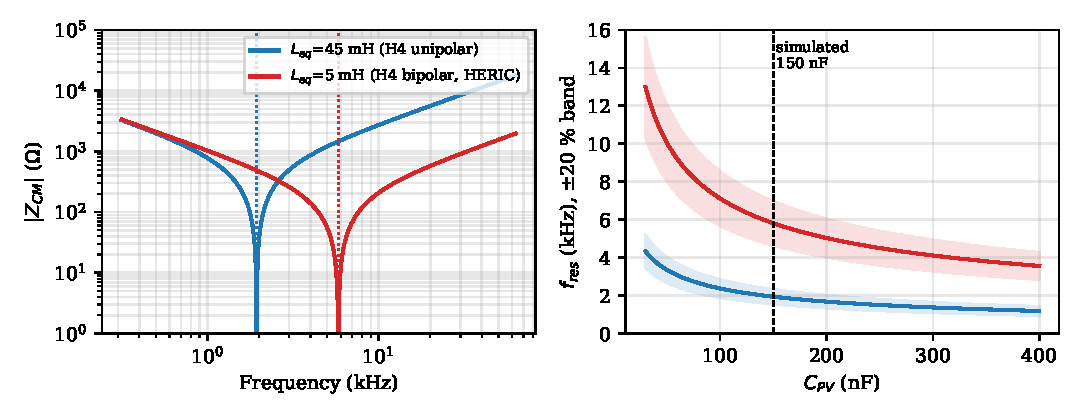
\includegraphics[width=0.85\textwidth]{figures/resonance_sensitivity.pdf}
\caption{Analytical CM-loop characteristics from \eqref{eq:icm} (no simulation data). (a)~Magnitude of the CM impedance for $\Cpv=150$~nF; dotted lines mark $\fres$. (b)~Resonance frequency versus parasitic capacitance, with the $\pm20\%$ avoidance band of the selection rule shaded.}
\label{fig:sens}
\end{figure*}

\subsection{Sensitivity to the parasitic capacitance}
The parasitic capacitance of a PV array is not a fixed number: it depends on the module technology, the mounting structure and the surface conditions, and increases when the module surface is wet \cite{Gubia2007,Khan2020}\todo{confirm that the cited sources give typical capacitance ranges before quoting numbers; none are quoted here}. Because $\fres\propto\Cpv^{-1/2}$, a doubling of $\Cpv$ lowers $\fres$ by 29\%. Table~\ref{tab:sens} lists the resonance for several values of $\Cpv$ together with the $\pm20\%$ avoidance bands for the two filter settings. The value of 330~nF is included only as a numerical example of a large capacitance.

\begin{table}[!t]
\renewcommand{\arraystretch}{1.2}
\caption{Resonance frequency and $\pm20\%$ avoidance band for varying $\Cpv$ (analytical, from \eqref{eq:icm})}
\label{tab:sens}
\centering
\footnotesize
\begin{adjustbox}{max width=\columnwidth}
\begin{tabular}{ccccc}
\toprule
 & \multicolumn{2}{c}{$\Leq=45$~mH} & \multicolumn{2}{c}{$\Leq=5$~mH} \\
\cmidrule(lr){2-3}\cmidrule(lr){4-5}
$\Cpv$ (nF) & $\fres$ (kHz) & Band (kHz) & $\fres$ (kHz) & Band (kHz) \\
\midrule
50  & 3.36 & 2.69--4.03 & 10.07 & 8.06--12.08 \\
100 & 2.37 & 1.90--2.84 & 7.12  & 5.70--8.54 \\
150 & 1.94 & 1.55--2.33 & 5.81  & 4.65--6.97 \\
300 & 1.37 & 1.10--1.64 & 4.11  & 3.29--4.93 \\
330 & 1.31 & 1.05--1.57 & 3.92  & 3.14--4.70 \\
\bottomrule
\end{tabular}
\end{adjustbox}
\end{table}

Two consequences follow. First, a switching frequency selected to avoid $\fres$ at 150~nF may fall into the avoidance band at a different capacitance: for the 5-mH filter, a design at $\fsw=7$~kHz is safe at 150~nF but is at the center of the band for 100~nF. The robust choice is $\fsw>2.4\fres$ evaluated for the \emph{smallest} expected $\Cpv$ (which gives the highest $\fres$); for $\Leq=5$~mH and $\Cpv=50$~nF this is $\fsw>24$~kHz. Second, a larger inductance moves $\fres$ down at the cost of a larger voltage drop: the 90-mH filter of the H4 unipolar case has $X_L/R_L>1$ (Table~\ref{tab:params}), which is much more than the 10\% rule of thumb for the voltage drop would permit, so the low $\fres$ of this case is partly a consequence of an oversized filter.

\subsection{Design procedure}
The results suggest the following procedure for selecting the switching frequency of a transformerless inverter with an L filter.
\begin{enumerate}
  \item Determine the bounds of $\Cpv$ for the installation (module technology, mounting, humidity), and compute $\fres$ from \eqref{eq:icm} at both bounds.
  \item Mark the avoidance bands $0.8\fres<k\fsw<1.2\fres$ for $k=1,2,3$ and $1.6\fres<\fsw<2.4\fres$ over the whole range of $\Cpv$.
  \item Choose $\fsw$ outside all bands and, if the efficiency target permits, above $2.4\fres$ evaluated at the smallest $\Cpv$.
  \item Verify with a time-domain simulation that the RMS leakage is below 300~mA and that the sudden changes of residual current remain below the steps of the standard \cite{IEC62109}; account for the effect of the switch output capacitances and dead time on the CMV.
  \item Check the efficiency and the filter ripple $\Delta I_{pp,\max}$ at the selected $\fsw$ with a loss model that includes the switching loss.
\end{enumerate}
Step~5 is essential: the sweeps in this paper do not capture the rise of the switching loss with $\fsw$, so the upper bound of the admissible frequency remains to be determined by a loss model or by measurement.

\subsection{Worked example}
Consider the H4 bipolar case ($L_1=L_2=10$~mH, $\Leq=5$~mH) installed on an array whose parasitic capacitance is expected to lie between 100~nF (dry) and 300~nF (wet). From Table~\ref{tab:sens}, $\fres$ lies between 4.11~kHz and 7.12~kHz, and the $\pm20\%$ bands on $\fsw$ for $k=1,2,3$ are $3.3$--$8.5$~kHz, $1.6$--$4.3$~kHz and $1.1$--$2.8$~kHz, respectively,
together with the band $6.6$--$17.1$~kHz around $2\fres$. Taken together over the range of $\Cpv$, these exclude $1.1~\text{kHz}<\fsw<17.1~\text{kHz}$, and the criterion $\fsw>2.4\fres$ at the smallest capacitance gives $\fsw>17.1$~kHz. The sweep of Fig.~\ref{fig:sweepH4B} (taken at 150~nF) shows that the leakage at 20 and 40~kHz is 60 and 14~mA, respectively, both well below the limit, and the choice between them is a matter of efficiency and ripple: 20~kHz has the lower switching loss but a ripple of $\Delta I_{pp,\max}=0.58$~A (about 1.5\% of the load-current amplitude), whereas 40~kHz reduces the ripple to 0.29~A. A design at 14~kHz, which the simple criterion $\fsw>2\fres$ would have allowed, falls inside the $2\fres$ band for the smallest-capacitance case and should be rejected. This example illustrates that the rule excludes a wide range for a poorly known $\Cpv$ and thus favors the upper part of the swept range or an inductance that places $\fres$ well below the intended $\fsw$.

\subsection{Experimental validation plan}
The results of this paper are simulation-based and the resonance rule should be validated on hardware before being relied upon. A minimal plan comprises (i) a single-phase H4/HERIC prototype in the 0.5--1~kW range with interchangeable L, LC and LCL filters and a selectable switching frequency; (ii) an emulated PV array in which a film capacitor bank of 50--330~nF is connected between the negative DC rail and the protective earth, replacing the unknown capacitance of real modules and allowing $\fres$ to be moved on purpose; (iii) measurement of $\iCM$ with a wide-band current probe in the earth lead and of the pole voltages, over the same frequency sweep as in simulation, with the RMS value compared with the 300~mA limit and the sudden steps with the limits of Table~\ref{tab:limits}; (iv) measurement of the efficiency with a power analyzer to bound the upper end of the admissible $\fsw$; and (v) an impedance measurement of the actual array (LCR meter between the shorted array terminals and the frame, dry and wet) to compare the measured $\Cpv$ with the assumed one. The comparison of the measured and predicted peak positions would directly test the first-order model \eqref{eq:icm}, whose neglect of loop resistance and of the ground-path inductance is the most important modeling assumption.
